\subsection{Modelo de Dados}

\par O modelo de dados reúne, no PostgreSQL, os usuários e as sessões, o cadastro, o histórico e os demais dados operacionais, como mostra a Figura~\ref{fig:cap3_modelo_dados}.

\begin{figure}[H]
    \centering
    \caption{Modelo de Dados}
    \label{fig:cap3_modelo_dados}
    \vspace{0.4cm}
    \resizebox{\textwidth}{!}{%
    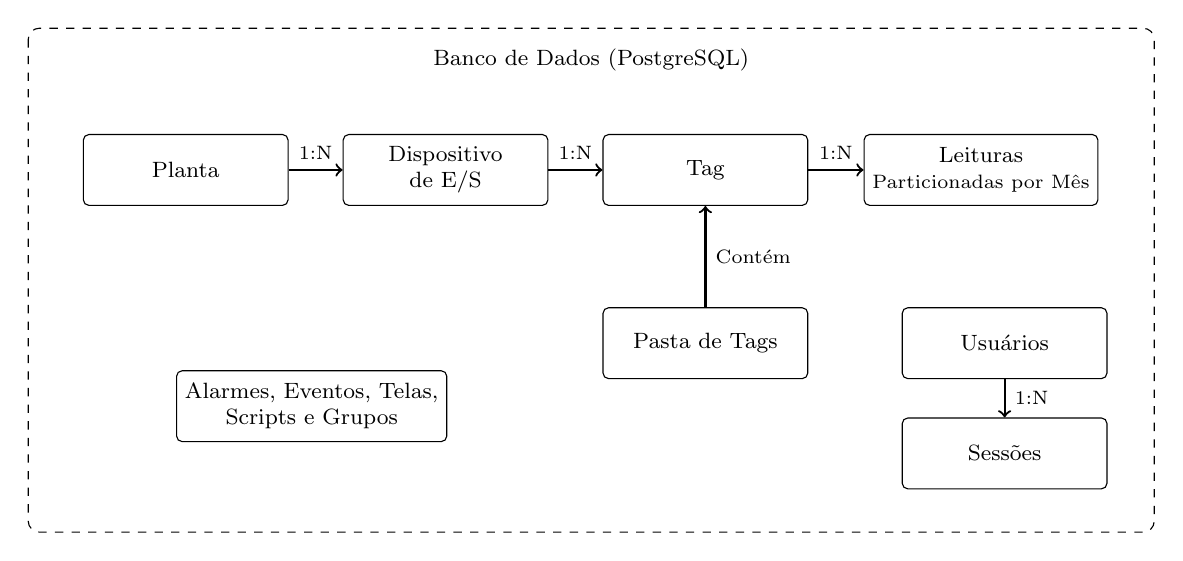
\begin{tikzpicture}[
        box/.style={draw, rounded corners=2pt, minimum width=2.6cm, minimum height=0.9cm, align=center, font=\footnotesize, fill=white, inner sep=3pt},
        conn/.style={->, thick}]
        \draw[dashed, rounded corners=4pt] (-0.4,3.0) rectangle (13.9,-3.4);
        \node[font=\footnotesize] at (6.75,2.6) {Banco de Dados (PostgreSQL)};
        \node[box] (pla) at (1.6,1.2) {Planta};
        \node[box] (dis) at (4.9,1.2) {Dispositivo\\de E/S};
        \node[box] (tag) at (8.2,1.2) {Tag};
        \node[box] (lei) at (11.7,1.2) {Leituras\\{\scriptsize Particionadas por Mês}};
        \node[box] (pas) at (8.2,-1.0) {Pasta de Tags};
        \node[box] (out) at (3.2,-1.8) {Alarmes, Eventos, Telas,\\Scripts e Grupos};
        \node[box] (usr) at (12.0,-1.0) {Usuários};
        \node[box] (ses) at (12.0,-2.4) {Sessões};
        \draw[conn] (pla) -- (dis) node[midway, above, font=\scriptsize] {1:N};
        \draw[conn] (dis) -- (tag) node[midway, above, font=\scriptsize] {1:N};
        \draw[conn] (tag) -- (lei) node[midway, above, font=\scriptsize] {1:N};
        \draw[conn] (pas) -- (tag) node[midway, right, font=\scriptsize] {Contém};
        \draw[conn] (usr) -- (ses) node[midway, right, font=\scriptsize] {1:N};
    \end{tikzpicture}}
    \vspace{0.2cm} \\
    Fonte: Autor.
\end{figure}

\par O cadastro tem três níveis. A planta é a instalação física, com nome, identificador textual e coordenadas para o mapa. O dispositivo de E/S é a origem do dado, um equipamento Modbus ou um dispositivo interno, que gera valores calculados ou simulados, e define o período de varredura. A tag é a variável monitorada ou comandada e traz o endereço do registrador, o tipo de dado, a ordem de bytes, a escala e a banda morta. Uma árvore de pastas própria de cada planta organiza as tags para a visualização, e uma pasta pode reunir tags de dispositivos diferentes.

\par As leituras formam a maior tabela do sistema, dividida por mês, e as partições futuras são criadas por tarefas de manutenção. Para períodos longos, há médias por minuto, usadas quando o período de varredura é inferior a sessenta segundos, e por hora. O banco guarda também alarmes, eventos, telas, listas de acompanhamento, scripts, variáveis meta, grupos e o registro de comandos, com a cópia do nome de quem os emitiu.

\par A exclusão de registros do cadastro é definitiva, e em vez de excluir é possível desabilitar um item.

